
\documentclass[a4paper]{article}
\usepackage[text={165mm,245mm}]{geometry}
\usepackage{graphicx}
\usepackage{subfigure}
\usepackage{ctex}
\usepackage{float} 
\usepackage{amsmath}
\usepackage{listings}
\usepackage{xcolor}
\definecolor{mygreen}{rgb}{0,0.6,0}  
\definecolor{mygray}{rgb}{0.5,0.5,0.5}  
\definecolor{mymauve}{rgb}{0.58,0,0.82}  
  
% RISC-V Assembler syntax and style for latex lstlisting package
% 
% These are risc-v commands as per our university (University Augsburg, Germany) guidelines.
%
% Author: Anton Lydike
%
% This code is in the public domain and free of licensing
\lstdefinelanguage[RISC-V]{Assembler}
{
  alsoletter={.}, % allow dots in keywords
  alsodigit={0x}, % hex numbers are numbers too!
  morekeywords=[1]{ % instructions
    lb, lh, lw, lbu, lhu,
    sb, sh, sw,
    sll, slli, srl, srli, sra, srai,
    add, addi, sub, lui, auipc,
    xor, xori, or, ori, and, andi,
    slt, slti, sltu, sltiu,
    beq, bne, blt, bge, bltu, bgeu,
    j, jr, jal, jalr, ret,
    scall, break, nop
  },
  morekeywords=[2]{ % sections of our code and other directives
    .align, .ascii, .asciiz, .byte, .data, .double, .extern,
    .float, .globl, .half, .kdata, .ktext, .set, .space, .text, .word
  },
  morekeywords=[3]{ % registers
    zero, ra, sp, gp, tp, s0, fp,
    t0, t1, t2, t3, t4, t5, t6,
    s1, s2, s3, s4, s5, s6, s7, s8, s9, s10, s11,
    a0, a1, a2, a3, a4, a5, a6, a7,
    ft0, ft1, ft2, ft3, ft4, ft5, ft6, ft7,
    fs0, fs1, fs2, fs3, fs4, fs5, fs6, fs7, fs8, fs9, fs10, fs11,
    fa0, fa1, fa2, fa3, fa4, fa5, fa6, fa7
  },
  morecomment=[l]{;},   % mark ; as line comment start
  morecomment=[l]{\#},  % as well as # (even though it is unconventional)
  morestring=[b]",      % mark " as string start/end
  morestring=[b]'       % also mark ' as string start/end
}
% language definition

\lstset{ %  
  backgroundcolor=\color{white},   % choose the background color; you must add \usepackage{color} or \usepackage{xcolor}  
  basicstyle=\footnotesize,        % the size of the fonts that are used for the code  
  breakatwhitespace=false,         % sets if automatic breaks should only happen at whitespace  
  breaklines=true,                 % sets automatic line breaking  
  captionpos=bl,                    % sets the caption-position to bottom  
  commentstyle=\color{mygreen},    % comment style  
  deletekeywords={...},            % if you want to delete keywords from the given language  
  escapeinside={\%*}{*)},          % if you want to add LaTeX within your code  
  extendedchars=true,              % lets you use non-ASCII characters; for 8-bits encodings only, does not work with UTF-8  
  frame=single,                    % adds a frame around the code  
  keepspaces=true,                 % keeps spaces in text, useful for keeping indentation of code (possibly needs columns=flexible)  
  keywordstyle=\color{blue},       % keyword style  
  %language=Bin,                 % the language of the code  
  morekeywords={*,...},            % if you want to add more keywords to the set  
  numbers=left,                    % where to put the line-numbers; possible values are (none, left, right)  
  numbersep=5pt,                   % how far the line-numbers are from the code  
  numberstyle=\tiny\color{mygray}, % the style that is used for the line-numbers  
  rulecolor=\color{black},         % if not set, the frame-color may be changed on line-breaks within not-black text (e.g. comments (green here))  
  showspaces=false,                % show spaces everywhere adding particular underscores; it overrides 'showstringspaces'  
  showstringspaces=false,          % underline spaces within strings only  
  showtabs=true,                  % show tabs within strings adding particular underscores  
  stepnumber=1,                    % the step between two line-numbers. If it's 1, each line will be numbered  
  stringstyle=\color{orange},     % string literal style  
  tabsize=2,                       % sets default tabsize to 2 spaces  
  %title=myPython.py                   % show the filename of files included with \lstinputlisting; also try caption instead of title  
}  
\title{\heiti 
CODH - 综合实验 \hspace{0.3cm}实验报告}
\author{院系: \kaishu\underline{}\hspace{1.5cm}姓名: \kaishu \underline{}\hspace{1.5cm}学号: \kaishu \underline{}\hspace{1.5cm}}
\begin{document}
\maketitle

\section{实验目的}
\begin{itemize}
    \item 掌握Cache基本原理、结构、设计和调试方法
    \item 掌握CPU输入/输出的编址和控制方式
    \item 熟练掌握数据通路和控制器的设计和描述方法
    
\end{itemize}

\section{实验环境}
\begin{itemize}
  \item macOS 13.0
  \item Rars1\_5.jar (Riscv Assembler and Runtime Simulator)
  \item Vivado 2019.3
  \item Nexys 4 DDR 开发板
\end{itemize}
\section{实验内容}
\subsection{Dcache与Dmem}
\begin{itemize}
    \item 熟练掌握数据通路和控制器的设计和描述方法
    \item 将原来的数据存储器改为Dmem,假定按块访问,首字读取延迟16个时钟,随后每字1个时钟
    \item 添加缓存Dcache,要求使用直接/二路组相连实现,采用写回写分配策略
    \item Dcache与CPU,Dcache与Dmem之间都使用Ready/Valid实现
\end{itemize}

  \subsection{IOU}
  \begin{itemize}
    \item CPU使用存储器映射的方式输入输出以对外设进行访问
    \item 主要的IO端口有:led,switch,btn,seg等
    \item 采用查询式输出过程和查询式输入过程
    \item 通过开关输入数据,LED及数码管输出显示
  \end{itemize}

  \subsection{测试程序}
  \begin{itemize}
    \item 使用IOU输入数组大小以及数组首元素
    \item 通过LFSR算法生成出数组其他元素
    \item 利用之前的排序代码排序,并检查排序结果是否正确。
    \item 排序前后计算所用时钟周期数
  \end{itemize}
\section{逻辑设计 / 核心代码}
\subsection{Dcache与Dmem的实现}
首先计算地址格式,要求Dmem总容量4KB,设置块大小为4字,因此1块=4字=16byte=128位,总共分为256块,
块地址应该有8位,字地址应该有8+2=10位。

使用IP核例化相应存储器后,在其上添加一层以满足实验需求。

在这里Dmem使用了FSM来实现,分为七个状态:IDLE,DELAY,WRITE,WT\_RDY,READ,RD\_RDY,FINISH。

初始Dmem处于IDLE状态,在读/写的valid信号有效后,进入DELAY状态模拟延时16个时钟周期,然后进入相应的
读写状态,读写完成后置相应的ready位有效,再次经由FINISH状态回到IDLE状态。

\begin{lstlisting}[language={verilog},title={Dmem.v}] 
    if(~rstn) begin
        state <= IDLE;
        r_ready <= 0;
        w_ready <= 0;
        delay_cnt <= 0;
        offset_cnt <= 0;
        wt_en <= 0;
    end
    else begin
        case(state)
            IDLE: begin
                if(w_valid || r_valid) begin
                    r_ready <= 0;
                    w_ready <= 0;
                    state <= DELAY;
                end
                else begin
                    r_ready <= 0;
                    w_ready <= 0;
                    state <= IDLE;
                end
            end
            DELAY: begin 
                if(delay_cnt < CYCLE) begin //wait 16 cycles
                    delay_cnt = delay_cnt + 1;
                    offset_cnt <= 0;
                end
                else begin
                    if(w_valid) begin
                        delay_cnt <= 0;
                        offset_cnt <= 0;
                        wt_en <= 1;
                        state <= WRITE;
                    end
                    else if(r_valid) begin
                        delay_cnt <= 0;
                        offset_cnt <= 1;
                        rd_addr <= {r_addr, offset_cnt[1:0]};
                        state <= READ;
                    end
                end
            end
            WRITE: begin
                if(offset_cnt < WORD_SIZE - 1)begin
                    //wt_data = ...
                    wt_en <= 1;
                    offset_cnt <= offset_cnt + 1;
                end
                else begin
                    offset_cnt <= 0;
                    wt_en <= 0;
                    state <= WT_RDY;
                end
            end
            WT_RDY: begin
                w_ready <= 1;
                state <= FINISH;
            end
            READ: begin
                wt_en <= 0;
                if(offset_cnt < WORD_SIZE) begin
                    rd_addr <= {r_addr, offset_cnt[1:0]};
                    r_data <= {dout, r_data[127:32]}; // 0, 
                    offset_cnt <= offset_cnt + 1;
                end
                else begin
                    r_data <= {dout, r_data[127:32]};
                    offset_cnt <= 0;
                    state <= RD_RDY;
                end
            end
            RD_RDY: begin
                r_ready <= 1;
                state <= FINISH;
            end
            FINISH: begin
                r_ready <= 0;
                w_ready <= 0;
                wt_en <= 0;
                state <= IDLE;
            end

        endcase
    end
\end{lstlisting}

接下来是Dcache,对地址进行分析,应该有\texttt{addr[9:0] = {tag[9:7], index[6:2], offset[1:0]}}
我们首先实现的是二路组相连Dcache,后期实现直接映射Cache时只需要修改地址格式并且将附加装置去掉即可。

Dcache的整体设计,参考了普通班的文档,但因为实际要求不同做了些许修改,主要核心是两个寄存器作为cache,两个寄存器作为tag,以及两个记录寄存器分别
记录dirty以及valid。除此之外控制信号的产生还需要有相应的FSM,写回时需要选路的基于LRU的选择器,以及写入cache时的数据插入器(cache是4字,但是Dcache每次写入是1字,需要插入相应位置)。

\begin{figure}[H]
    \centering
    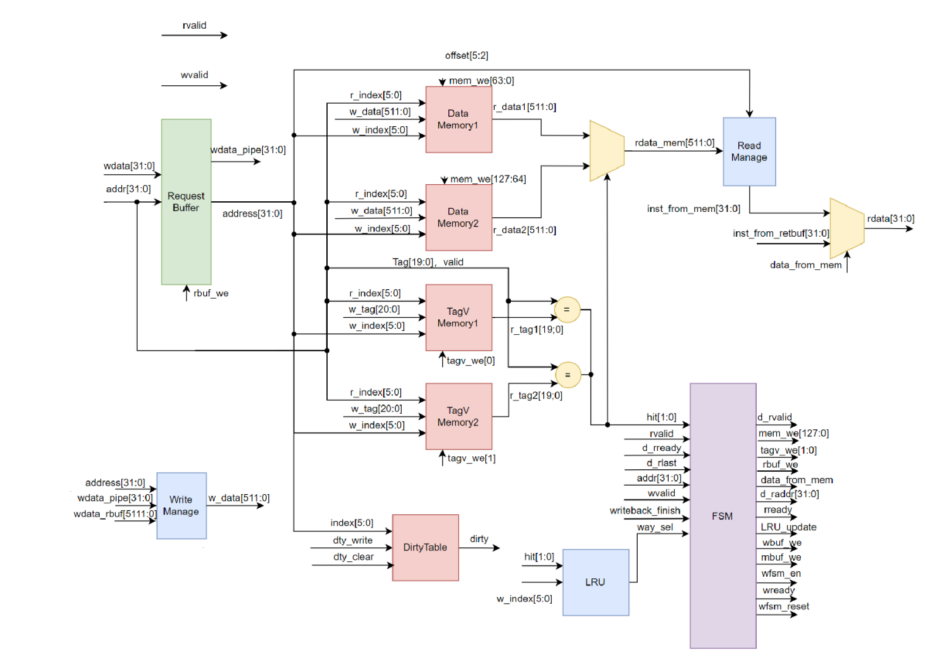
\includegraphics[width=1.0\textwidth]{1.png}
    \caption{CPU-fig}
    \label{fig:Dmem}
\end{figure}

Dcache还有一个重点是FSM的设计,这里参照了书本上的简化FSM实现。主要分为IDLE,WRITE\_BACK,FETCH,FINISH几个阶段。

初始Dcache处于IDLE状态,当CPU发出读/写请求时,根据地址计算出tag以及index,然后根据index去cache中查找,如果命中则进入下一周期就置ready,仍然停留在IDLE状态。
否则需要替换cache,先检查LRU选择的cache块是否dirty,若是则进入WRITE\_BACK将块写回Dmem,若不是则进入FETCH阶段直接
fetch所需要读写的块,然后在FINISH阶段对cache块中的数据进行读写,置ready位有效并跳回IDLE状态。

具体代码如下
\begin{lstlisting}[language={verilog},title={fsm.v}] 
    case (state) 
        IDLE: begin
            if (w_valid || r_valid) begin 
                if (hit) begin //stay IDLE
                    //更新 LRU
                    LRU_change <= 0;
                    LRU_update <= 1;
                    if(w_valid) begin
                        w_data_sel <= 0; // w_data_write = (w_word + r_data)
                        dty_write <= 1;
                        w_ready <= 1;
                        r_ready <= 0;
                        if(hit1) begin 
                            mem_we1 <= 1;
                            tag_we1 <= 0;
                        end
                        else if (hit2) begin 
                            mem_we2 <= 1;
                            tag_we2 <= 0;
                        end
                        state <= FINISH;
                    end
                    else if(r_valid) begin 
                        data_from_mem <= 0;
                        dty_write <= 0;
                        r_ready <= 1;
                        w_ready <= 0;
                        valid_write <= 0;
                        mem_we1 <= 0;
                        mem_we2 <= 0;
                        tag_we1 <= 0;
                        tag_we2 <= 0;
                        state <= IDLE;
                    end
                end
                else begin //miss
                    LRU_change <= 0;
                    LRU_update <= 0;
                    w_ready <= 0;
                    r_ready <= 0;
                    dty_clear <= 0;
                    dty_write <= 0;
                    valid_write <= 0;
                    mem_we1 <= 0;
                    mem_we2 <= 0;
                    tag_we1 <= 0;
                    tag_we2 <= 0;
                    if(dirty) begin
                        dw_valid <= 1;
                        dr_valid <= 0;
                        state <= WRITE_BACK;
                    end
                    else begin
                        dr_valid <= 1;
                        dw_valid <= 0;
                        state <= FETCH;
                    end
                end
            end
            else begin //stay IDLE
                LRU_change <= 0;
                LRU_update <= 0;
                w_ready <= 0;
                r_ready <= 0;
                state <= IDLE;
            end
        end
        WRITE_BACK: begin
            LRU_change <= 0;
            LRU_update <= 0;
            if(~dw_ready) begin
                dw_valid <= 1;
                dr_valid <= 0;
                state <= WRITE_BACK;
            end
            else begin
                dw_valid <= 0;
                dr_valid <= 1;
                state <= FETCH;
            end
        end
        FETCH: begin
            if(~dr_ready) begin
                dr_valid <= 1;
                dw_valid <= 0;
                state <= FETCH;
            end
            else begin//写入新的tag,data,dirty,LRU,读取完成
                if(valid[way_sel]) begin
                    LRU_change <= 1;
                    LRU_update <= 0;
                end
                else begin
                    LRU_change <= 0;
                    LRU_update <= 0;
                end
                dr_valid <= 0;
                dw_valid <= 0;

                w_data_sel <= 1;

                mem_we1 <= way_sel ? 0 : 1;
                mem_we2 <= way_sel ? 1 : 0;
                tag_we1 <= way_sel ? 0 : 1;
                tag_we2 <= way_sel ? 1 : 0;

                w_ready <= 1;
                r_ready <= 1;
                if (~w_valid) begin
                    dty_clear <= 1;
                    dty_write <= 0;
                end
                else  begin
                    dty_clear <= 2;
                    dty_write <= 0;
                end
                valid_write <= 1;
                data_from_mem <= 1;
                state <= FINISH;
            end
        end
        FINISH: begin
            data_from_mem <= 0;
        w_data_sel <= 0;
        LRU_update <= 0;
        LRU_change <= 0;
        dty_clear <= 0;
        dty_write <= 0;
        valid_write <= 0;
        mem_we1 <= 0;
        mem_we2 <= 0;
        tag_we1 <= 0;
        tag_we2 <= 0;
        w_ready <= 0;
        r_ready <= 0;
            state <= IDLE;
        end
        endcase
\end{lstlisting}

Dcache的正确性通过专门编写的汇编程序进行了测试,这个汇编程序尝试写入数据到index相同地址不同的3块,并且再读出数据,
以此来检查Dcache能否正确写回以及LRU选择是否正确。汇编程序如下:
\begin{lstlisting}[language={[RISC-V]Assembler},title={test.asm}] 
.text
main:
    addi t1, zero, 1
    slli a0, t1, 13
    sw t1, 0(a0)
    addi t1, t1, 1
    addi a0, a0, 4
    sw t1, 0(a0)
    addi t1, t1, 1
    addi a0, a0, 4
    sw t1, 0(a0)
    addi t1, t1, 1
    addi a0, a0, 4
    sw t1, 0(a0)
    
    addi a0, zero,1
    slli a0, a0, 13
    addi a0, a0, 0x100
    addi a0, a0, 0x100
    addi t1, t1, 1
    sw t1, 0(a0)
    addi a0, a0, 4
    
    addi t1, t1, 1
    sw t1, 0(a0)
    addi a0, a0, 4
    
    addi t1, t1, 1
    sw t1, 0(a0)
    addi a0, a0, 4
    
    addi t1, t1, 1
    sw t1, 0(a0)
    
    addi t1, t1, 1
    addi a0, zero, 1
    slli a0, a0, 13
    addi a0, a0, 0x100
    addi a0, a0, 0x100
    addi a0, a0, 0x100
    addi a0, a0, 0x100
    addi t1, t1, 1
    sw t1, 0(a0)
    addi a0, a0, 4
    
    addi t1, t1, 1
    sw t1, 0(a0)
    addi a0, a0, 4
    
    addi t1, t1, 1
    sw t1, 0(a0)
    addi a0, a0, 4
    
    addi t1, t1, 1
    sw t1, 0(a0)
    
    addi a0, zero,1
    slli a0, a0, 13
    lw t1, 0(a0)
    lw t1, 4(a0)
    lw t1, 8(a0)
    lw t1, 12(a0)
    

    
    
    
end: jal end
\end{lstlisting}

\subsection{IOU}
这一部分相对Dcache比较简单,主要工作量在于需要实现比较繁琐的各个相应外设部件的代码。

首先对于输入,要将按钮信号去抖动;对于开关要实现数码管实时显示编辑数据,每次拨动开关输入一个16进制数字,按下del按钮删去一个数字,按下data按钮
完成数据编辑。这一部分主要是编码的工作,开关编辑数据的核心代码如下
\begin{lstlisting}[language={verilog},title={switch\_data.v}] 
always@(posedge clk)
begin
    if(~rstn || btnc) 
    begin
        tmp <= 0;
    end
    else if(p && !btnr)
    begin
        tmp <= (tmp << 4) + h; 
    end
    else if(!p && btnr)
    begin
        tmp <= tmp >> 4;
    end
end
\end{lstlisting}

每当收到开关信号产生变化时,在别的模块中会开始去边沿,并将处理完成的数据以及一个时钟周期的有效位给到switch\_data模块中,在这里将其加入数据的最后一位。

对于IOU的主体部分,简单的数据将地址对应的外设寄存器读出/写入即可。

比较复杂的部分即是开关数据以及七段数码管的查询时输入输出,具体逻辑如下:当数码管准备好时,rdy置1;可以输出到数码管显示数据,此时rdy置0(数码管忙);
用户查看完显示数据后按下按钮,rdy再次置1。开关数据编辑好前,swx\_rdy置0,按下按钮后置1,此时CPU可以读入开关数据,读入完成后将swx\_rdy置0,数据清零,等待下一次编辑。
核心代码如下:
\begin{lstlisting}[language={verilog},title={IOU.v}] 
    always @(posedge clk) begin    //CPU输出
    if (~rstn) begin
        led_data <= 16'hFFFF;
        seg_data <= 32'h12345678;
    end
    else if (io_we) begin
        case (io_addr)
            8'h00:
                led_data <= io_dout;
            8'h0C:
                seg_data <= io_dout;
            default: ;
        endcase
    end
end


always @(posedge clk) begin
    if (~rstn)
        seg_rdy <= 1;
    else if (io_we & (io_addr == 8'h0C))
        seg_rdy <= 0;
    else if (BTNU_P || BTNL_P || BTND_P)
        seg_rdy <= 1;
end


always @(posedge clk) begin
    if (~rstn)
        swx_vld <= 0;
    else if (BTNC_P & ~swx_vld) begin
        swx_data <= tmp;
        swx_vld <= 1;
    end
    else if (io_rd & (io_addr == 8'h14))
        swx_vld <= 0;
end

always@(posedge clk) begin
    if(~rstn)
        cnt_data <= 32'h0;
    else
        cnt_data <= cnt_data + 32'h1;
end

always @(*) begin  
    case (io_addr)
        8'h04:
            io_din = {{11{1'b0}}, BTNC_P, BTNU_P, BTNL_P, BTNR_P, BTND_P, sw};
        8'h08:
            io_din = {{31{1'b0}}, seg_rdy};
        8'h10:
            io_din = {{31{1'b0}}, swx_vld};
        8'h14:
            io_din = swx_data;
        8'h18:
            io_din = cnt_data;
        default:
            io_din = 32'h0;
    endcase
end
\end{lstlisting}

\subsection{汇编测试代码}
相较之前的代码只添加了IOU输入数据以及使用LFSR生成的部分,代码如下,其中LFSR采用[9 5 0]的本原多项式。
\begin{lstlisting}[language={[RISC-V]Assembler},title={test.asm}]
    loop: 
    beq t0, zero, sort_wait
    sw t1, 0(t5)

    addi t2, zero, 1 #t2 -> 0x1
    slli t2, t2, 9
    and t3, t1, t2    #t3 = t1[9]
    srli t3, t3, 9    #-> [0]

    # addi t2, zero, 0x1 //t2 -> 0x1
    srli t2, t2, 3
    and t4, t1, t2    # t4 = t1[5]
    srli t4, t4, 6    

    addi t2, zero, 1 
    sub t0, t0, t2
    xor t3, t3, t4
    xor t3, t3, t2   # t3 = t1[9] ^ t1[5] ^ 1
    slli t3, t3, 11

    srli t1, t1, 1
    add t1, t1, t3  # t1 = {t3, t1 >> 1}

    addi t5, t5, 4
    jal loop
\end{lstlisting}  

最后的测试部分通过简单的遍历所有数据并且判断是否前一项大于后一项,如果不是则说明排序失败,否则说明排序成功。

若排序成功,将会在LED输出0x40,否则输出0x20,通过查看LED即可判断排序是否成功。

\subsection{CPU的修改}
CPU的部分不用修改太多,只需要将之前的data\_mem替换为IOU和Dcache的结合体即可,根据地址选择IOU或是Dcache进行响应。

除此之外,还修改了stall部分,当数据读写valid时,若ready信号没有产生,则需要stall整个CPU。

CPU的修改详见cpu.v

烧录后测试程序以及排序程序的正确性已经由助教检查完成,综合设计任务至此完成。

\subsubsection{结果分析}
RTL电路:
\begin{figure}[H]
    \centering
    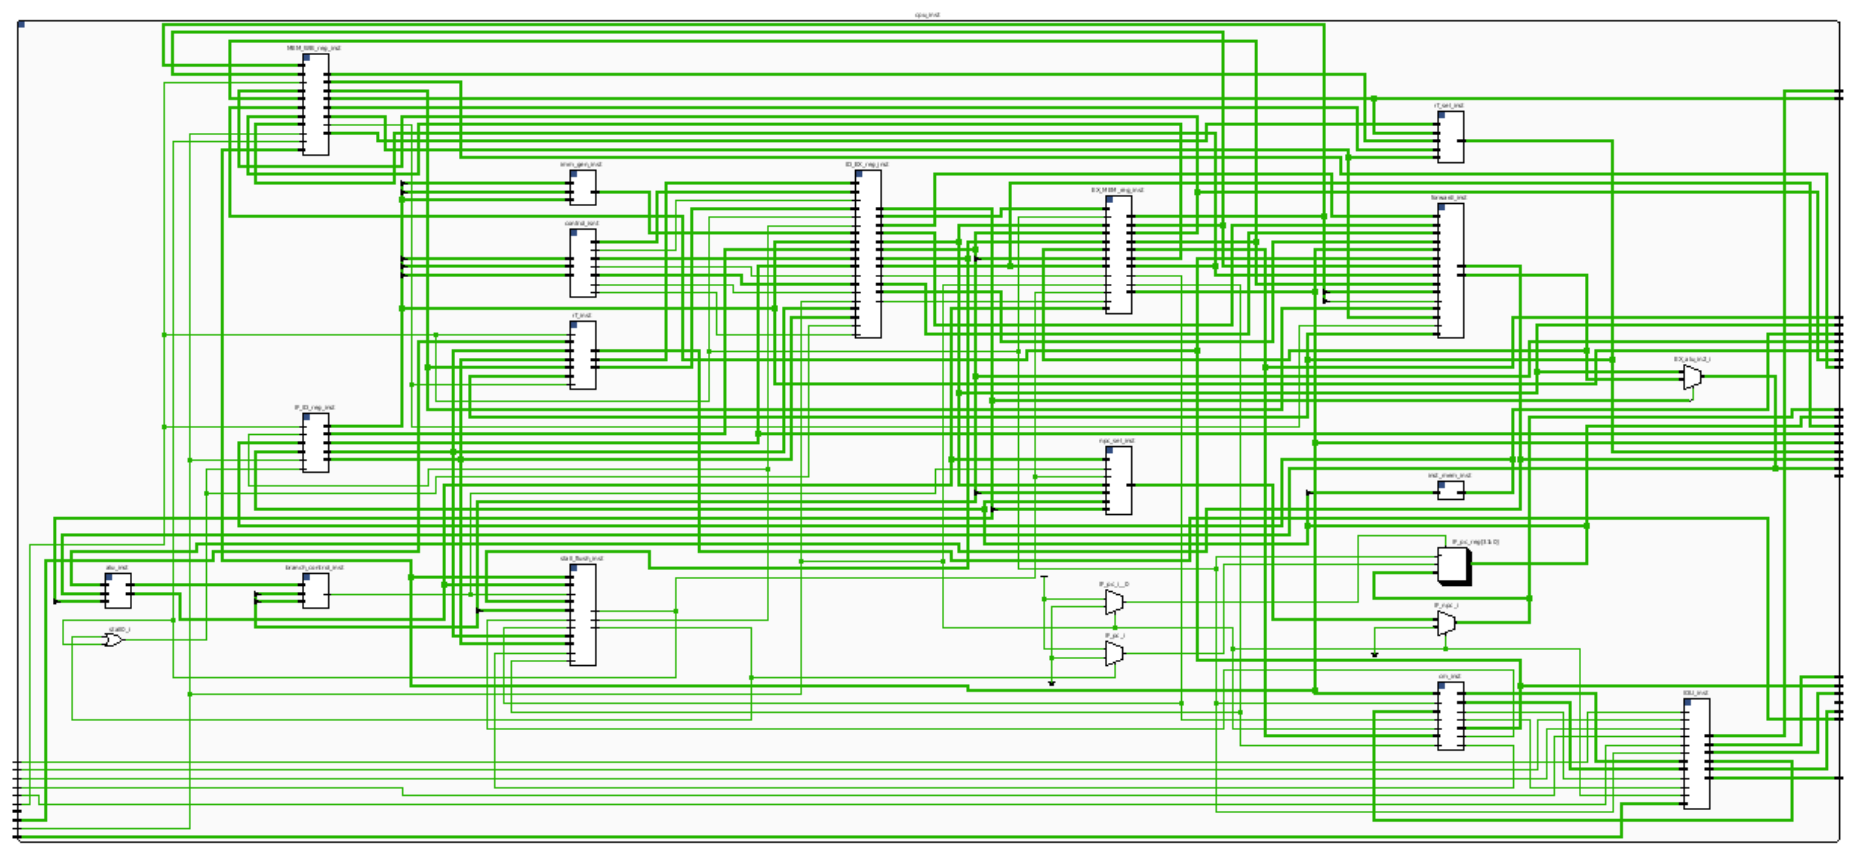
\includegraphics[width=0.9\textwidth]{3.png}
    \caption{RTL}
    \label{fig:test1}
\end{figure}

电路资源使用情况:
\begin{figure}[H]
    \centering
    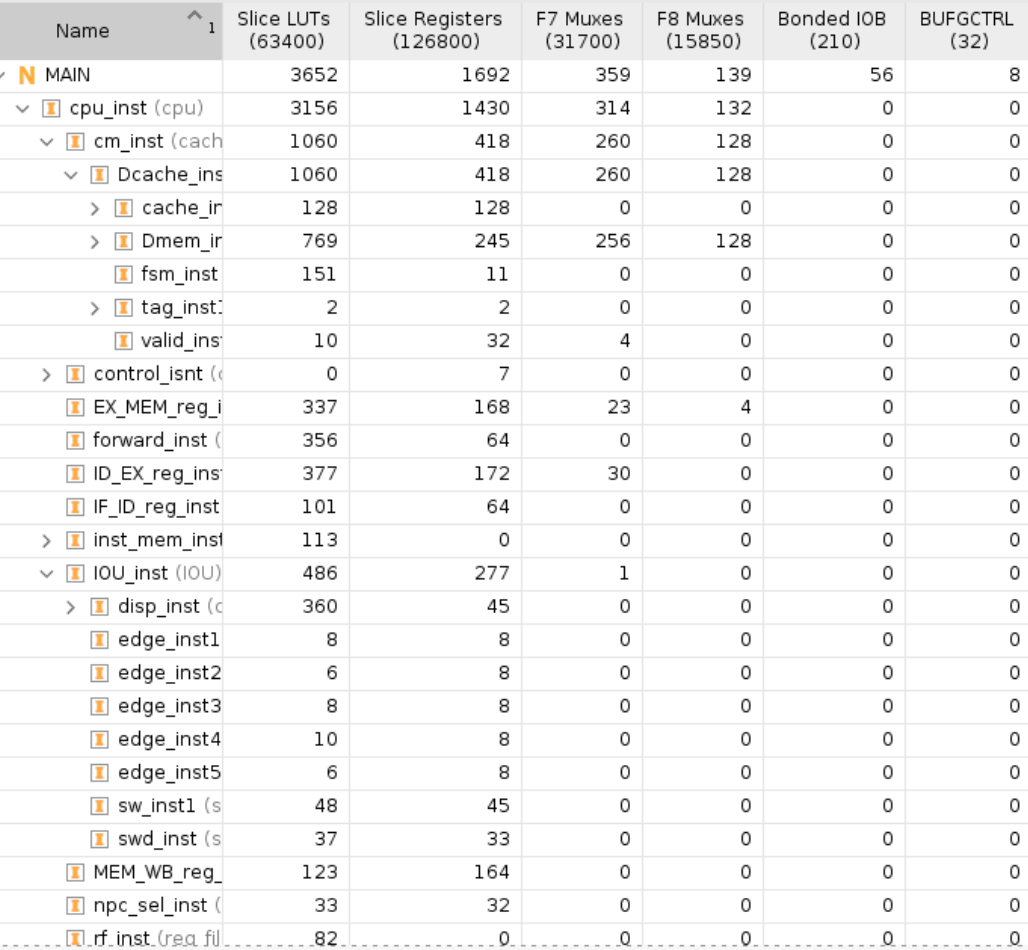
\includegraphics[width=0.9\textwidth]{2.png}
    \caption{UTL1}
    \label{fig:test1}
\end{figure}


电路性能:
\begin{figure}[H]
    \centering
    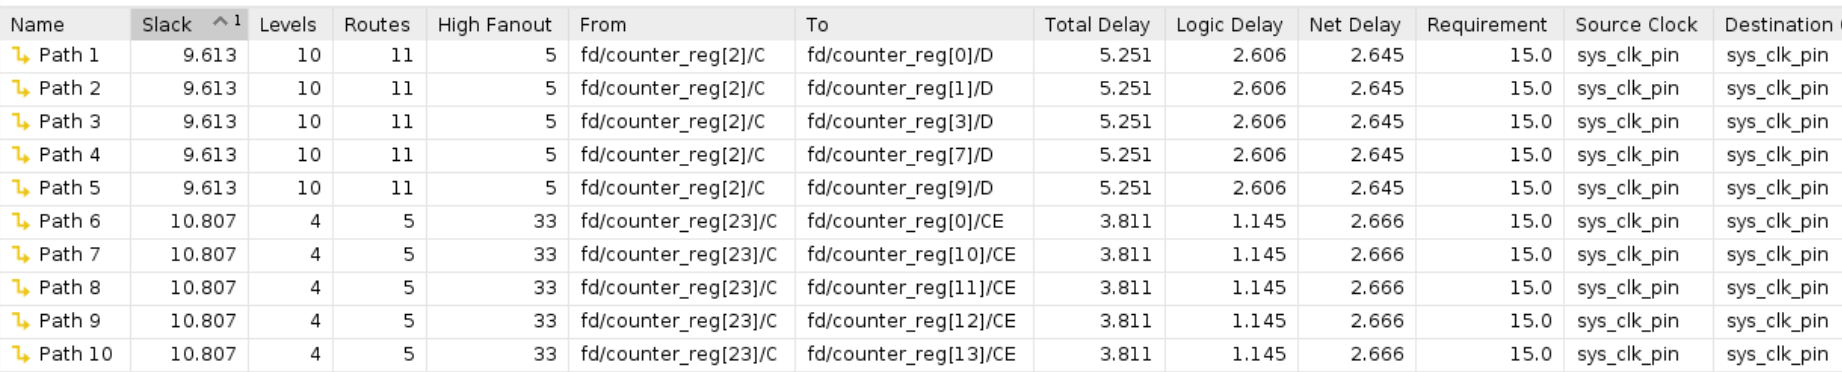
\includegraphics[width=0.9\textwidth]{4.png}
    \caption{TIMING}
    \label{fig:test1}
\end{figure}

\section {实验总结}
\begin{enumerate}
  \item 通过本次实验,我学习到了如何依据需求修改流水线CPU的数据通路来增加功能,比如cache和IOU
  \item 通过本次实验,我理解了如何通过地址映射以及IOU组件使CPU与外设进行交互,还有查询式输入输出的实现方法
  \item 通过本次实验,我学习了Dcache的各个模块如何具体设计,以及FSM的编写方法。学习到了先设计再编写的重要性
\end{enumerate}
\section {意见/建议}
    实验过于复杂,文档要求含糊不清,而且教学部分几乎为0。希望能够改进。
\end{document}